\chapter{Synchronizing}

Synchronization refers to coordinating the actions of multiple processes that share resources.

In short, it involves the coordination of processes that access shared resources
\begin{itemize}
   \item Needs for avoiding inconsitencies or conflicts
   \begin{itemize}
      \item Prevent conflicts and inconsistencies that
      arise when multiple processes access
      shared data or resources concurrently.
   \end{itemize}
   \item Managing access to shared resources
   \begin{itemize}
      \item In a way that maintains data integrity and
      system performance.
   \end{itemize}
\end{itemize}

In Distributed Systems the communication happens through networks and message passing among multiple independent proceses.
\labelitemize{Challenges}{
   \begin{enumerate}
      \item Network Delays - Variable communication times may lead to inconsistencies
      \item Process Failures - Processes may fail at any time, so their failure must be handled
      \item No Fairness - We must preventing starvation or indefinite delays for processes waiting to access resources.
   \end{enumerate}
}

\section{Mutual Exclusion}
Mutual exclusion is a well-known \textbf{solution} to access shared resources in a distributed system, avoiding interferences.

\begin{definition}
   [Mutual Exclusion]
   A property that ensures only one process can enter a critical section at any given time.
\end{definition}
The \textbf{Critical section} is a portion of code accessing shared resources.

In other words, Mutual Exclusion enforces \textbf{atomical} access to shared resources, avoiding conflicts and inconsistencies.
Note that \textit{atomic} does not imply the hardware support for atomic operations, we use it as a logical and semantical concept.

\framedt{Mutual Exclusion Goals}{
   \begin{itemize}
      \item \textbf{Safety} - Only one process can access the critical section at a time
      \item \textbf{Liveness} - Ensures that every process that wishes to enter the critical section will eventually be able to do so, preventing starvation.
      \item \textbf{Fairness} - Requests for entry to the critical section are granted in the order they are made, ensuring no process is perpetually denied access.
   \end{itemize}
}


\subsection{Types of Mutual Exclusion}
\begin{enumerate}
   \item \textbf{Software-based} - Algorithms such as Lamport's Bakery Algorithm, Peterson's Algorithm, Dekker's Algorithm, etc.
   \item \textbf{Hardware-based} - Atomic operations or locks
   \item \textbf{Hybrid approaches} - Combining software and hardware-based solutions to achieve better performance and reliability.
\end{enumerate}

\begin{figure}[htbp]
   \centering
   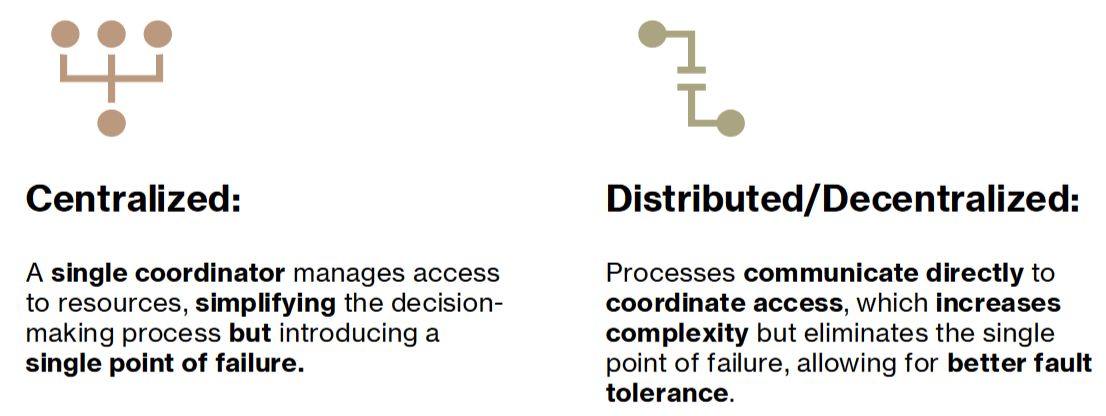
\includegraphics{images/04/mutual_types.png}
   \caption{Mutual exclusion - Centralized vs Distributed}
   \label{fig:04/mutual_types}
\end{figure}

\subsection{LBA - Lamport's Bakery Algorithm}
LBA is a software-based mutual exclusion algorithm that uses a ticket system to ensure fairness and prevent starvation.
LBA simulates a bakery where customers take a number and are served in order, clearly the processes are the customers.

\begin{enumerate}
   \item A process picks a ticket number that is one greater than the maximum ticket number currently in use.
   \item The process waits until all processes with smaller ticket numbers have completed their critical sections.
   \item The process with the lowest ticket number enters the critical section.
   \item The process resets its ticket number to indicate it has finished.
\end{enumerate}

It is \textbf{unlikely} for two processes to pick the same ticket number due to the sequential nature of ticket assignment, but it is possible.

In the rare cases where multiple processes attempt to obtain a ticket simultaneously, they may end up with the same number. To solve this the algorithm specifies that the process with the smaller identifier (\texttt{pid}) has priority ensuring fairness among competing processes.

The process enters the critical section only after verifying that no other process with a smaller ticket number is currently in the critical section.
Once the process completes its operations in the critical section, it releases its ticket by resetting its number to zero. The reset indicates to other processes that the critical section is available.

\begin{lstlisting}[language=C]
   choosing[N] -> {false, false, ..., false} // Initialize choosing flags for each process
   number[N] -> {0, 0, ..., 0} // Initialize ticket numbers for each process
   ...
   Process (i):
      lock(i);
         critical session code
      unlock(i);

   void lock(int i) {
      choosing[i] = true;
      number[i] = 1 + max(number[0], ..., number[N-1]);
      choosing[i] = false;
      for (int j = 0; j < N; j++) {
         while (choosing[j]); // Wait until other processes have chosen
         while (number[j] != 0 && (number[j] < number[i] || (number[j] == number[i] && j < i)));
      }
   }
\end{lstlisting}

Note that unlike some hardware-based synchronization mechanisms (like spinlocks or test-and-set instructions), LBA does not require atomic operations or specific CPU instructions. Besides, LBA relies on simple ticketing logic and does not depend on hardware features, it can be implemented in various environments, enhancing its portability.

Its major \textbf{drawback} is that it may suffer from performance issues (e.g., high communication overhead) in large systems due to continuous polling of ticket values.
However, it nicely environments where shared memory is available and the number of processes is relatively small.

\subsection{LDMEA - Lamport's Distributed Mutual Exclusion Algorithm}
LDMEA is a distributed version of Lamport's Bakery Algorithm that allows processes to access shared resources across multiple nodes, exploiting logical clocks for coordination.

\begin{figure}[htbp]
   \centering
   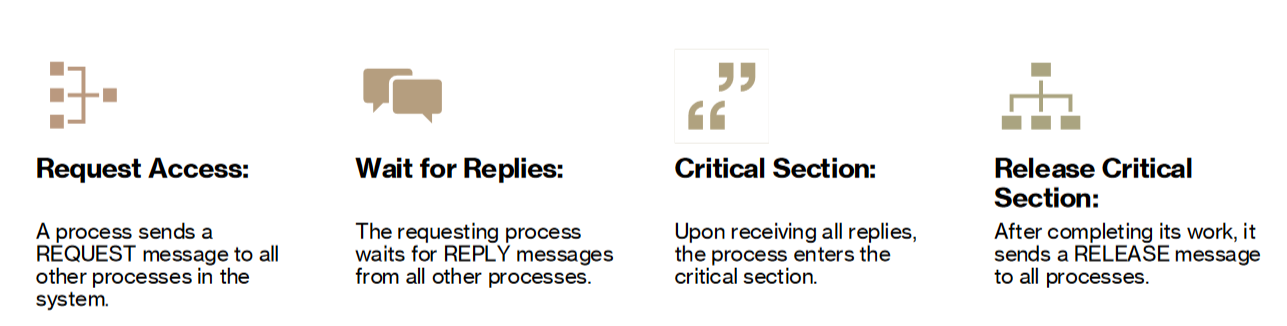
\includegraphics{images/04/ldmea_steps.png}
   \caption{LDMEA Key Steps}
   \label{fig:04/ldmea_steps}
\end{figure}

Each process maintains a logical clock to timestamp its requests, which is incremented at each request or receive.
Requests are ordered based on their logical timestamps, and the process with the smallest timestamp is granted access to the critical section.

Every site $S_i$, keeps a queue to store critical section requests ordered
by their timestamps. $request\_queue_i$ denotes the queue of site $S_i$.

\subsubsection{Entering the Critical Section}
When a site $S_i$ wants to enter the critical section, it sends a request message $Request(ts_i, i)$ to all other sites and places the request on $request\_queue_i$. Here, $Ts_i$ denotes the timestamp of Site $Si$.
A site $S_i$ can enter the critical section if it has received the message with timestamp larger than $(ts_i, i)$ from all other sites and its own request is at the top of $request_queue_i$

\subsubsection{Leaving the Critical Section}
When a site $S_i$ leaves the critical section, it removes its own request from the top of its request queue and it sends a release message $Release(ts_i, i)$ to all other sites and removes its request from $request_queue_i$.

When a site $S_j$ receives the timestamped RELEASE message from site $S_i$, it removes the request of $S_i$ from its request queue.

\subsubsection{Considerations and drawbacks}
\labelitemize{Example}{
   \begin{enumerate}
      \item \textbf{P1} sends a \texttt{REQUEST} message with its
      timestamp to \textbf{P2} and \textbf{P3}.
      \item \textbf{P2} and \textbf{P3} reply to \textbf{P1}.
      \item Once \textbf{P1} receives all \texttt{REPLY} messages, it
      enters the critical section.
      \item After finishing, \textbf{P1} sends a \texttt{RELEASE}
      message to \textbf{P2} and \textbf{P3}
   \end{enumerate}
}

Wrapping up we need
\begin{itemize}
   \item (N - 1) request messages
   \item (N - 1) reply messages
   \item (N - 1) release messages
\end{itemize}
So, the first drawback is that LDMEA incurs a high number of messages (3n) for each entry into the critical section. 
Besides, LDMEA also has to handle \textbf{failures}: requires additional mechanisms to handle process failures and network partitions.

However, the message passing in LDMEA, aside from making it suitable for distributed systems, even though it introduces overhead, it is still better than the polling mechanism in LBA, where processes have to continuously check for ticket values.